\section{Modess - Modal Effective Sound Speed}
\label{sec: Modess}

{\bf Modess} implements a normal mode expansion for propagation of a single tone in a stratified atmosphere in the effective sound speed approximation. Recall that in the effective sound speed approximation the influence of the atmospheric winds is approximated by adding the along-path component of the horizontal winds to the sound speed and then propagating through the resulting effective sound speed, $c_{eff}$, as if there were no wind. This approximation is valid for sufficiently low angle propagation paths and sufficiently low wind speeds (low Mach numbers). Attenuation by the atmosphere, implemented via the addition of an attenuation coefficient as the imaginary part of the wave number, is taken into account as a perturbation. The perturbative treatment of the atmospheric attenuation produces accurate results for tropospheric and stratospheric ducting, and for frequencies low enough that attenuation is not significant, but generally should not be considered accurate for signals returned from the thermosphere. The ground surface is assumed to be rigid. 

\subsection{Mathematical Background}
\label{sec: modess math}

Let $z$ denote altitude above the ground surface and let the subscript $H$ denote horizontal displacement. Let $r=\|\textbf{x}_{H}\|$ be the radial horizontal range. Let $\rho_0$ be the mean density of the atmosphere, let $\alpha$ be the atmospheric attenuation coefficient, $\omega$ the angular frequency, and $p$ the deviation from mean pressure at horizontal position $\textbf{x}_{H}$ and altitude $z$. Then {\bf Modess} solves the following generalized Helmholtz equation: 
\begin{equation}
\Big[ 
\nabla_{H}^2
+
\rho_0 \frac{\partial}{\partial z} \Big(\frac{1}{\rho_0} \frac{\partial}{\partial z} \Big)  
+
\Big(\frac{\omega}{c_{eff}(z)} + i\alpha (\omega,z)\Big)^2 
\Big] p(r,z,\omega) = 0. 
\label{eq: eff c Helmholtz}
\end{equation}
The pressure deviation $p$ satisfies the boundary condition 
\[
\frac {\partial p}{\partial z}\Big |_{z=0}= 0
\]
on the ground surface. If the signal source is assumed to be at zero range, $r=0$, and altitude $z_S$ then $p$ is asymptotic, for small distance $r,(z-z_S)\downarrow 0$, to the field produced by a unit acoustic source, 
\[
\lim_{r,(z-z_S)\downarrow0}\Big(p(r,z,\omega)-\frac{1}{\sqrt{r^2+(z-z_S)^2}}\Big)=0.
\]

The solution is obtained by the method of normal modes, see e.g. \cite{comp_oc_ac}. Computed is the modal sum for the far field pressure deviation 
\begin{equation}
p(r,z,\omega)
\approx
\frac{e^{i \pi /4}}{\sqrt{8 \pi r}} \sqrt{\frac {\rho_0(z)} {\rho_0(z_s)}} \sum_j\psi_j(z_s)\psi_j(z) \frac{e^{i (k_j+i\alpha_j)r}}{\sqrt{k_j}}
\label{eq: modess far field pressure}
\end{equation}
where the modal wave numbers $k_j$ and mode functions $\psi_j$ are real valued and $k_j^2$ are the eigenvalues and $\psi_j$ the corresponding eigenfunctions of the eigenvalue problem 
\[
\Big( 
\frac{d^2}{dz^2} +\frac{\omega^2}{c_{eff}^2}
\Big)\psi(z) 
= 
k^2\psi(z) 
\quad \text{with} \quad 
\psi^\prime(0)=0. 
\]
Note that terms related to buoyancy have been dropped. The modal attenuation coefficients $\alpha_j$ are estimated using leading order perturbation theory, see e.g. \cite{Landau_QM}. One finds 
\[
\alpha_j=c_j\int_0^\infty \frac{\alpha(\omega,z)}{c_{eff}(z)}\ (\psi_j(z))^2\, dz. 
\]
Here $c_j=\frac{\omega}{k_j}$ is the modal phase velocity. 

The eigenvalue problem is solved by replacing the continuous vertical domain with a discrete grid, using finite differences to approximate the derivatives with respect to $z$, truncating the vertical domain at some large altitude, T, and then solving the resulting finite dimensional eigenvalue problem. A uniformly spaced grid, with spacing $h$, is used and a nearest neighbor centered difference approximation is used for the second derivative: 
\[
\frac{d^2f}{dz^2}\approx \frac{f(z-h)-2f(z)+f(z+h)}{h^2}. 
\]
The resulting matrix is of the form
\[
\textbf{M}
=
\frac{1}{h^2}\begin{pmatrix}
-1 - h^2\frac{\omega^2}{c_{eff}(0)^2} && 1 && 0 && \hdots && 0\\ \\
1 && -2 - h^2\frac{\omega^2}{c_{eff}(h)^2}&& 1 && \hdots && \vdots\\ \\
0 && 1 && -2  - h^2\frac{\omega^2}{c_{eff}(2h)^2}&& \hdots && \vdots\\ \\
\vdots && \vdots && \vdots && \ddots && 1 \\ \\
0 && \hdots && \hdots && 1 && -2  - h^2\frac{\omega^2}{c_{eff}(T)^2}
\end{pmatrix}.
\]
The eigenvalue problem reduces to a large dimensional linear algebra problem: find the eigenvalues $k^2$ and corresponding eigenvectors $\Psi$ that satisfy 
\[
M\Psi=k^2\Psi. 
\]

With this simple choice for the discrete approximation to the second derivative a very large number of vertical points are required, generally tens of thousands, to obtain accurate results; however, the resulting matrices are tridiagonal, allowing for extremely efficient numerical algorithms. The benefits of having tridiagonal matrices to diagonalize turns out to outweigh the problems encountered in dealing with the resulting large matrices. The number of vertical points required has been determined by checking that the results converge. Generally, the number increases with increasing frequency, but also with increasing complexity of the effective sound speed. The default is chosen to be 20,000, which has been found to be sufficient for the NCPA toy atmosphere up to about 5 Hz. 

\begin{figure}
\begin{center}
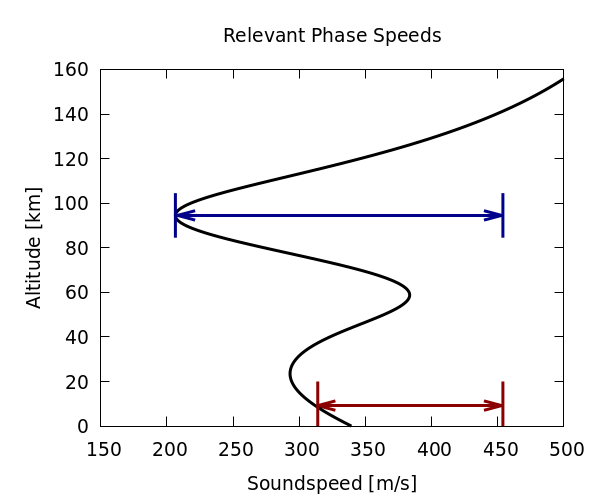
\includegraphics[width=0.45\textwidth]{figs/wvnums_modess}
\end{center}
\caption{Phase velocities used in {\bf Modess} for the NCPA toy atmosphere. The black curve is the effective sound speed for eastward propagation. The blue double-headed arrow shows the range of phase velocities needed in the modal sum. The red double-headed arrow shows the range of phase velocities needed for propagation to or from the ground. The minimum trace velocity is chosen so that all propagating modes are computed. The maximum trace velocity is chosen so that the modal sum converges in the far field. }
\label{fig:wvnums_modess}
\end{figure}

Only a relatively small subset of the eigenvalues of the approximating matrix \textbf{M} are needed for the modal sum. These correspond to the phase velocities (and hence modal wave numbers) needed for the evaluation and convergence of the modal sum. Modes can propagate in regions of the atmosphere where their phase velocities are greater than the effective soundspeed. It follows that only wave numbers whose corresponding phase velocities are greater than the minimum of the effective soundspeed need to be considered. The maximum phase velocity is chosen large enough to insure convergence of the modal sum. In practice one increases the maximum phase velocity until convergence is achieved. In {\bf Modess} one increases the maximum phase velocity by increasing the maximum altitude of the computational domain. 

These criteria are depicted graphically in Fig.\,\ref{fig:wvnums_modess} for eastward propagation in the NCPA toy atmosphere. The minimum phase velocity is chosen so that all propagating modes are included in the modal sum. If the source and receiver altitudes are to be arbitrary then the minimum phase velocity corresponds to the minimum of the effective sound speed. This is depicted by the blue arrows in the figure. If either the source or receiver are at zero altitude then fewer modes are required, as depicted by the red arrows. In this case the minimum phase velocity is determined by estimating the modal penetration to the ground in the WKB approximation. Once the relevant range of phase velocities, and thus of eigenvalues of \textbf{M}, has been determined the eigenvalues are computed using a Sturm alogorithm \cite{Stoer_Bulirsch} and the corresponding mode functions are obtained by the method of inverse iteration \cite{Press:2007:NRE:1403886}. 

Once the relevant wavenumbers and modes have been calculated, {\bf Modess} computes the modal sum Equ.\,\ref{eq: modess far field pressure} and then saves the resulting $p(r,z,\omega)$ to files. Note that $p(r,z,\omega)$ depends on azimuth through the effective sound speed. $p(r,z,\omega)$ will be referred to as the (complex valued) transmission loss despite the fact that transmission loss is more generally defined to be the negative of the magnitude of $p(r,z,\omega)$ expressed in dB relative to 1. In addition to the complex valued transmission loss, {\bf Modess} computes the incoherent transmission loss $I(r,z,\omega)$ defined by (see \cite{comp_oc_ac}) 
\[
I(r,z,\omega)
=
\frac{1}{\sqrt{8 \pi r}} \sqrt{\frac {\rho_0(z)} {\rho_0(z_s)}} \sqrt{\sum_j\frac{e^{-2\alpha_jr}}{k_j}\big(\psi_j(z_s)\psi_j(z)\big)^2\,} .
\]
The incoherent transmission loss is the mean transmission loss in the approximation that the relative phases of the modal contributions are random. It provides a simple approximation for an average transmission loss in a fluctuating atmosphere. 

\subsection{Running Modess}
\label{sec:running modess}

Making sure that the executable for {\bf Modess} is in the system's path, it can be run by entering 
\begin{verbatim} 
    Modess [--option1 val1] [--option2 val2] [...] [--flag1] [...] 
\end{verbatim}
on a command line. Generally, options are followed by values, either numbers, strings or filenames. Flags are not. Entering \verb"Modess --help" sends the following help page to the screen: 

\begin{verbatim}
By default the program computes the 1D transmission loss (TL) at the ground or
the specified receiver height and saves the data to 2 files:
    file tloss_1d.nm - considering attenuation in the atmosphere
    file tloss_1d.lossless.nm - no attenuation
Additionally, if the flag --write_2d_tloss is present on the command line, the
2D TL is saved to file tloss_2d.nm. The user can also choose to propagate in N
different directions i.e. (N by 2D mode) by using the option --multiprop.

The options below can be specified in a colon-separated file "modess.param" or
at the command line. Command-line options override file options.

Options Control:
  --help                 Prints help test
  --paramfile            Parameter file name [modess.param]
  --printparams          Print parameter summary to screen

Required Parameters:
  --atmosfile            Atmospheric profile filename
  --freq                 Frequency of analysis (Hz)

Optional Parameters [default]:
  --maxheight_km         Maximum height of analysis in km [150.0]
  --zground_km           Ground height [take from Z0 parameter in atmosfile, or
                         0.0]
  --Nz_grid              Number of vertical grid points to use [20000]
  --sourceheight_km      Source height in km [0.0]
  --receiverheight_km    Receiver height in km [0.0]
  --maxrange_km          Maximum range in km to use for modeling [1000.0]
  --Nrng_steps           Number of range steps to use [1000]
  --ground_impedence_model
                         Impedence model to use. Currently only "rigid" is
                         supported. [rigid]
  --use_attn_file        File name containing attenuation, to override default
                         Sutherland/Bass [n/a]. Columns are
                         Height(km) Attenuation(np/m)
  --modal_starter_file   Filename to output a starter file for the pape module
  --dispersion_file      Filename to output the dispersion information
    --append_dispersion_file
                         Append results to dispersion file rather than
                         overwriting

Modes of Operation:
  --singleprop           Single azimuth propagation. Requires --azimuth
    --azimuth            Azimuth of propagation, in degrees CW from North
                         [0,360)
  --multiprop            Multiple azimuth propagation. Requires --azimuth_start,
                         --azimuth_end, and --azimuth_step
    --azimuth_start      Starting azimuth, in degrees CW from North [0,360)
    --azimuth_end        Ending azimuth, in degrees CW from North [0,360)
    --azimuth_step       Azimuth step, in degrees CW from North [0,360)

Flags:
  --write_2d_tloss       Output 2-D transmission loss to tloss_2d.nm
  --write_phase_speeds   Output phase speeds to phasespeeds.nm
  --write_speeds         Output both the phase speeds and the group speeds to
                         speeds.nm
  --write_modes          Output modes to mode_###.nm. Also implies
                         --write_speeds
  --write_atm_profile    Output atmospheric profile to atm_profile.nm
  --Lamb_wave_BC         Use admittance = -1/2*dln(rho)/dz
  --turnoff_WKB          Turn off the WKB least phase speed estimation
  --wvnum_filter         Use wavenumber filter by phase speed. Requires --c_min
                         and --c_max
    --c_min              Minimum phase speed to keep
    --c_max              Maximum phase speed to keep



OUTPUT Files: Format description (column order):
  tloss_1d.nm:                 r, 4*PI*Re(P), 4*PI*Im(P), (incoherent TL)
  tloss_1d.lossless.nm:
  tloss_2d.nm:                 r, z, 4*PI*Re(P), 4*PI*Im(P)
  Nby2D_tloss_1d.nm:
  Nby2D_tloss_1d.lossless.nm:  r, theta, 4*PI*Re(P), 4*PI*Im(P), (incoherent TL)
  phasespeeds.nm:              Mode#, phase speed [m/s], imag(k)
  speeds.nm:                   Mode#, phase speed [m/s], group speed [m/s], imag(k)
  mode_<mode_count>.nm         z, (Mode amplitude)
  dispersion_<freq>.nm         Contains one line with entries:
                               freq, (# of modes), rho(z_src), rho(z_rcv)
                               followed for each mode 'i' by quadruples:
                               real(k(i)), imag(k(i)), Mode(i)(z_src), Mode(i)(z_rcv)
  atm_profile.nm               z,u,v,w,t,d,p,c,c_eff

Examples (run from 'samples' directory):
    ../bin/Modess --singleprop --atmosfile NCPA_canonical_profile_zuvwtdp.dat \
         --azimuth 90 --freq 0.1

    ../bin/Modess --singleprop --atmosfile NCPA_canonical_profile_zuvwtdp.dat \
         --azimuth 90 --freq 0.1 --write_2d_tloss

    ../bin/Modess --multiprop --atmosfile NCPA_canonical_profile_zuvwtdp.dat \
         --freq 0.1 --azimuth_start 0 --azimuth_end 360 --azimuth_step 1

\end{verbatim}

To use {\bf Modess} an ascii file containing the atmospheric specifications must be loaded using \verb+--atmosfile+ followed by the filename. {\bf Modess} always functions at a single frequency, specified using the \verb+--freq+ option. 

By default {\bf Modess} writes the transmission loss at a fixed azimuth as a function of range to a receiver on the ground, $p(r,0,\omega)$, to a file named \verb+tloss_1d.nm+; the azimuth must be specified using \verb+--azimuth+ followed by an angle in degrees. This is referred to as the 1D transmission loss. For use in testing and debugging, the lossless 1D transmission loss is also written to a file named \verb+tloss_1d.lossless.nm+. Receiver altitudes other than $z=0$ can be set by using the \verb+--receiverheight_km+ option. Similarly, the source altitude can be set using \verb+--sourceheight_km+. In general, \verb+tloss_1d.*+ files have four columns: range $r$, $\text{Re}\ p$, $\text{Im}\ p$, and incoherent transmission loss $I$. 

If the flag \verb+--write_2d_tloss+ is set then the 2D transmission loss, by which we understand the transmission loss as a function of range and altitude, is written to the file \verb+tloss_2d.nm+.  This file has four columns; $r$, $z$, $\text{Re}\ p$, $\text{Im}\ p$ in that order; written in line-separated blocks of constant $r$. The 2D transmission loss magnitude is useful in identifying the various propagation paths and their relative magnitudes. The propagation paths are obscured by the incoherent transmission loss and so is not very informative as a function of range and altitude and is not written to the file. 

The other flag that is directly related to propagation in \verb+--multiprop+. If this flag is set then the 1D transmission losses are calculated for a range of azimuths $\theta$ and then saved to the file \verb+Nby2Dtloss_1d.nm+ and \verb+Nby2Dtloss_1d.lossless.nm+. The range of azimuths is specified using the options \verb+--azimuth_start+, \verb+--azimuth_end+, and \verb+--azimuth_step+, each followed by an angle. \verb+--multiprop+ is used to model propagation from a source location to a portion of the horizontal plane, for a fixed receiver altitude. The files \verb+Nby2Dtloss_1d.*+ have five columns; $r$, $\theta$, $\text{Re}\ p$, $\text{Im}\ p$, and $I$; written in line separated blocks of constant $r$. If \verb+--multiprop+ is set then it is advised that \verb+--write_2d_tloss+ not be set. 

It is critical that \verb+--maxheight_km+ be less than the maximum altitude contained in the atmospheric specification file. Otherwise the program will crash. Most of the other options and flags are self explanatory. Exceptions are \verb+--ground_impedance_model+ which is designed to allow for an impedance boundary condition on the ground (this option is not yet supported), \verb+--Lamb_wave_BC+ followed by 0 or 1 which implements the Lamb wave impedance condition when it has the value 1 (this is the lowest order buoyant effect), \verb+--use_attn_file+ followed by a file name which allows the user to input an arbitrary attenuation profile through a user-supplied ascii file, and finally \verb+--modal_starter_file+ followed by a file name which writes a modal starter to the given file to be used with the package's PE model. 

\subsection{Running Modess: examples}
\label{sec: modess examples}

The \textbf{Modess} help page ends with three examples. The examples set the frequency to 0.1 Hz to keep run times short. The first is a simple example illustrating the primary input modes for Modess. It is assumed that the user runs it in the \verb+samples+ directory. Note that if the \textbf{ncpaprop} \verb+bin+ directory is in the system's path one may enter \verb+Modess+ rather than \verb+../bin/Modess+. The command line entry for the example is 
\begin{verbatim} 
    ../bin/Modess --singleprop --atmosfile NCPA_canonical_profile_zuvwtdp.dat \ 
                  --azimuth 90 --freq 0.1
\end{verbatim}
In this example the four required options are set. Otherwise the default settings are used. Ground-to-ground propagation in the NCPA toy atmosphere (see Figure \ref{fig:canonic_sound_speeds}) at 90 degrees azimuth (from North), eastward propagation, at frequency of 0.1 Hz is modelled. By default the signal is propagated out to 1000 km in range with range steps of 1 km. The atmospheric profiles are specified in the column-based text file \verb"NCPA_canonical_profile_zuvwtdp.dat" that is included in the \verb+samples+ directory. In the above example the profile file has 7 columns in the order \verb"zuvwtdp" (refer to section~\ref{sec: AtmoSpecs}  for an explanation of atmospheric specifications).

\begin{figure}[h]
\begin{center}
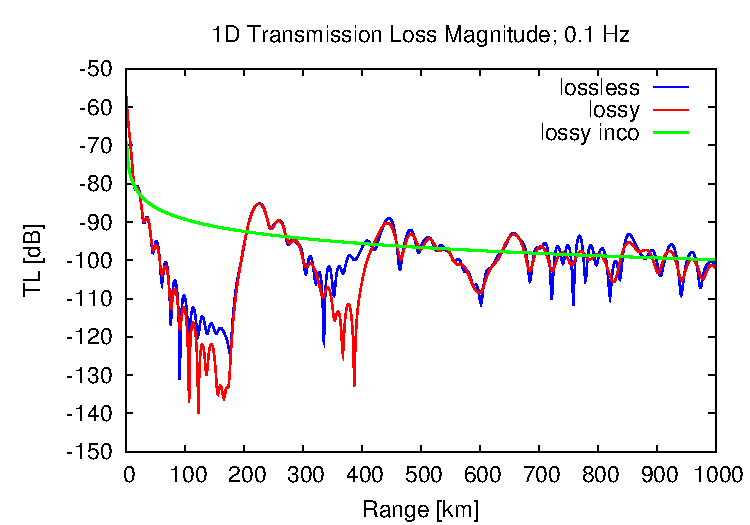
\includegraphics[scale=0.60]{figs/modess_ex1}
\end{center}
\caption{1D transmission loss magnitude at 0.1 Hz obtained with {\bf Modess} for eastward ground-to-ground propagation in the NCPA toy atmosphere shown in Figure \ref{fig:canonic_sound_speeds}. Shown are the lossless transmission loss magnitude, the lossy transmission loss magnitude and the lossy incoherent transmission loss.}
\label{fig: modess 1D tl}
\end{figure}

The output is, by default, the one-dimensional (1D) transmission loss on the ground for both lossy and lossless cases and is written into the text files \verb+tloss_1d.nm+ and \verb+tloss_1d.lossless.nm+ as described above in section~\ref{sec:running modess}.  An example of the magnitude of the complex 1D transmission loss output is shown in Figure \ref{fig: modess 1D tl}. Note that in general the output from all programs will be saved in the directory from which the code is run.  
\begin{figure}
\begin{center}
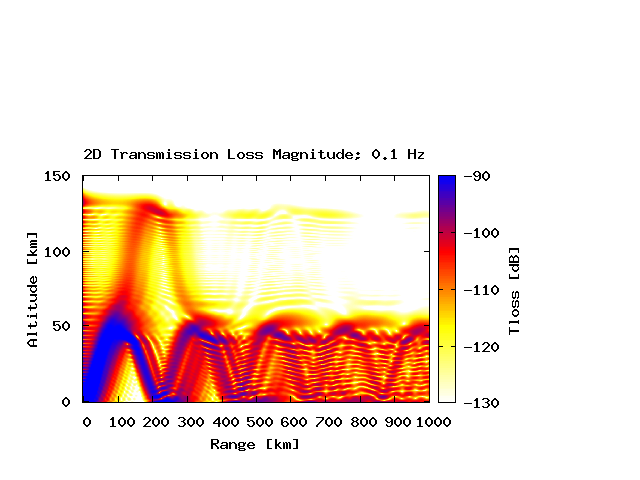
\includegraphics[width=0.6\textwidth]{figs/modess_ex2.png}
\end{center}
\caption{2D transmission loss magnitude at 0.1 Hz obtained with {\bf Modess} for eastward propagation in the NCPA toy model. The source is placed on the ground at the origin.}
\label{fig: modess 2D tl}
\end{figure}

In the second example the \verb+--write_2D_Tloss+ flag is appended to the command line entry for the first example: 
\begin{verbatim} 
    ../bin/Modess --singleprop --atmosfile NCPA_canonical_profile_zuvwtdp.dat \ 
                  --azimuth 90 --freq 0.1 --write_2d_tloss
\end{verbatim}
As described above in section~\ref{sec:running modess}, the output is written to the file \verb+tloss2d.nm+. The 2D transmission loss magnitude that results from eastward propagation in the NCPA toy model is plotted in Figure \ref{fig: modess 2D tl}. 
\begin{figure}
\begin{center}
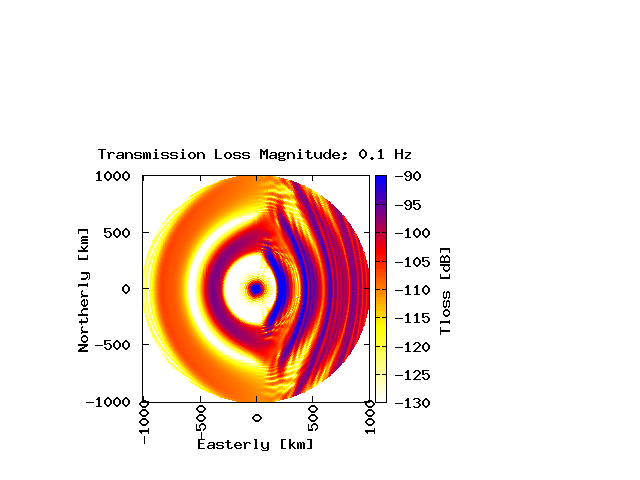
\includegraphics[width=0.4\textwidth]{figs/modess_ex3}\ 
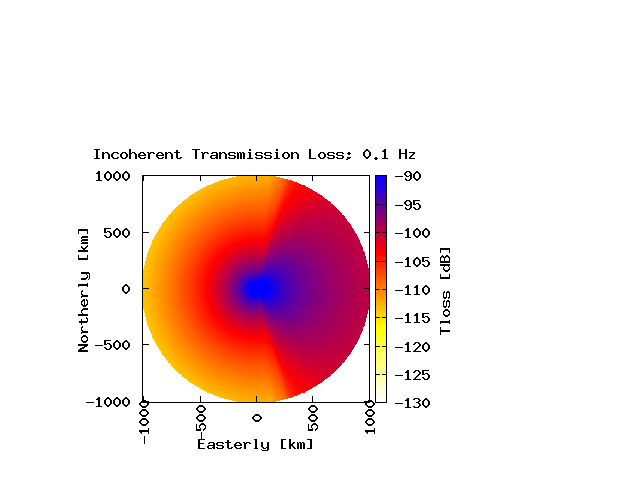
\includegraphics[width=0.4\textwidth]{figs/modess_ex3_inco}
\end{center}
\caption{N by 2D transmission loss magnitude and incoherent transmission loss obtained with {\bf Modess} for ground-to-ground propagation in the NCPA toy model atmosphere from a source at the origin to all azimuths.}
\label{fig: modess Nby2D tl}
\end{figure}

In the third example the \verb+--multiprop+ flag is appended to the command line entry for the first example. This flag requires that values for the options \verb+--azimuth_start+, \verb+--azimuth_end+, and \verb+--azimuth_step+ be given. The command line entry is 
\begin{verbatim} 
    ../bin/Modess --multiprop --atmosfile NCPA_canonical_profile_zuvwtdp.dat \
                  --freq 0.1 --azimuth_start 0 --azimuth_end 360 --azimuth_step 1
\end{verbatim}
The output is written to the files \verb+Nby2D_tloss_1d.nm+ and \verb+Nby2D_tloss_1d.lossless.nm+ as described above in section~\ref{sec:running modess}. The lossless transmission losses are also computed and saved as are the incoherent transmission losses and the resulting transmission loss magnitude is plotted in Figure \ref{fig: modess Nby2D tl}. 
\begin{figure}
\begin{center}
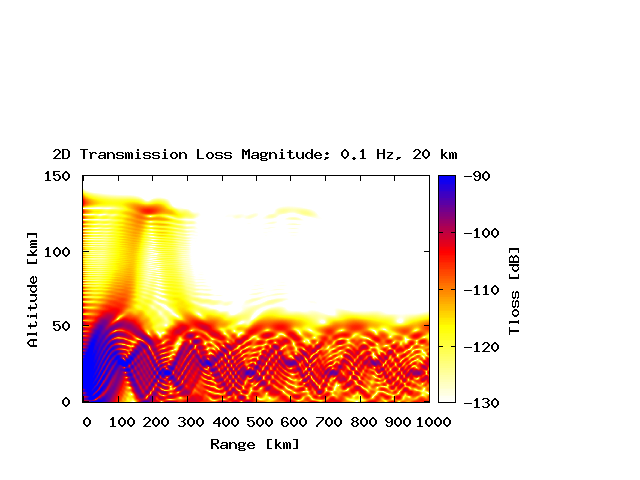
\includegraphics[width=0.6\textwidth]{figs/modess_ex2_20km_source}
\end{center}
\caption{2D transmission loss magnitude for propagation from an elevated source at 20 km altitude to the ground, obtained with {\bf Modess} for propagation in the NCPA toy atmosphere.}
\label{fig: modess 2D elevated source}
\end{figure}
A final example, not included in the \textbf{Modess} help page consider the calculation of a 2D transmission loss from an elevated source. For eastward propagation in the NCPA toy atmosphere from a source at 20 km altitude the command line entry is 
\begin{verbatim} 
    ../bin/Modess --singleprop --atmosfile NCPA_canonical_profile_zuvwtdp.dat \ 
                  --azimuth 90 --freq 0.1 --write_2d_tloss --sourceheight_km 20
\end{verbatim}
The resulting 2D transmission loss magnitude is plotted in Figure \ref{fig: modess 2D elevated source}. Note that the calculation only goes out to a range of 1 km. 
